In the framework of robotics for prosthetics, it is nowadays possible
to build mechanically advanced prostheses, such as mechanical hands
able to replicate a fair amount of the movements required by the
disabled to carry on living in a decent way.  Attempts in this sense
include, e.g., the DLR prosthetic hand (\cite{Hua2006} --- see Figure
\ref{fig:DLRHandII}), the CyberHand project \cite{cyberhand}, and the
i-LIMB hand by Touch Bionics \cite{ilimb}. Still, a general sense of
frustration impends, as far as control is concerned. How is an amputee
supposed to command the prosthesis what to do (i.e., how to grasp an
object) and with what force?

\begin{figure}
  \begin{tabular}{cc}
    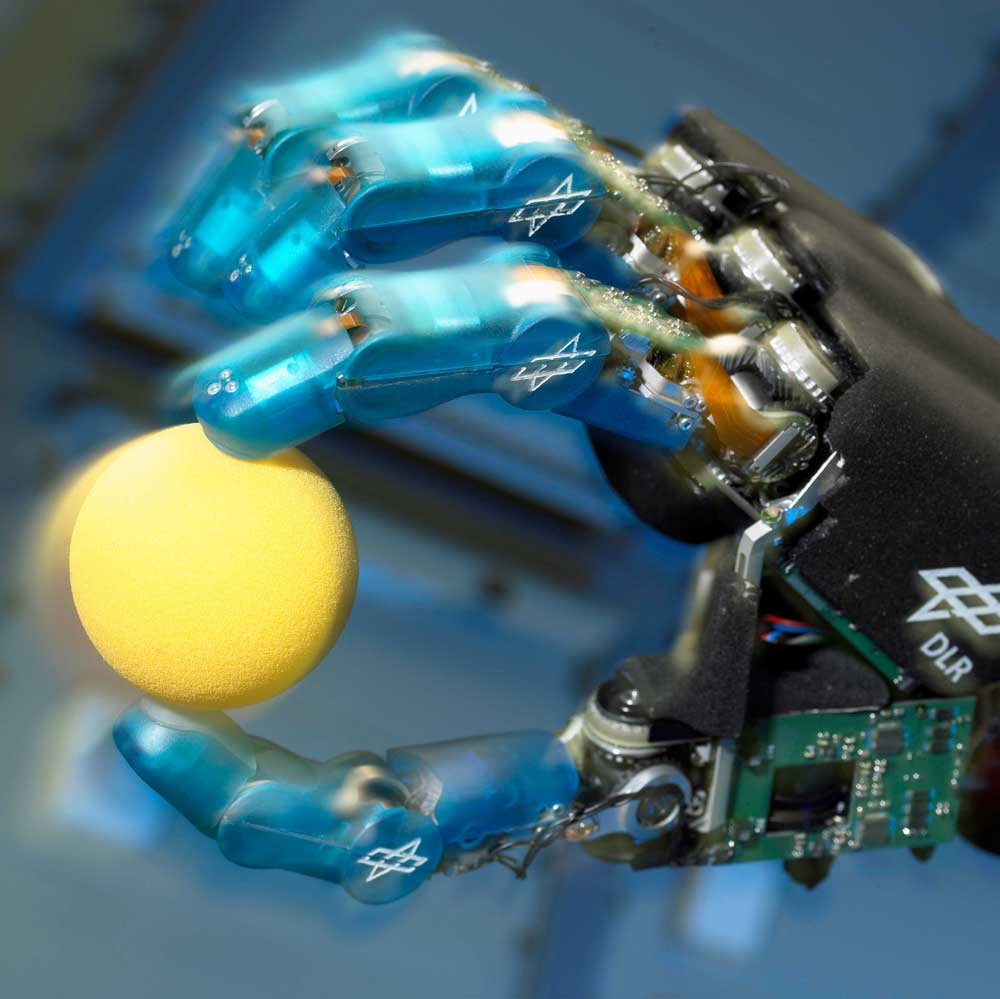
\includegraphics[height=3.3cm]{figs/DLRHand-Ball-comp} &
    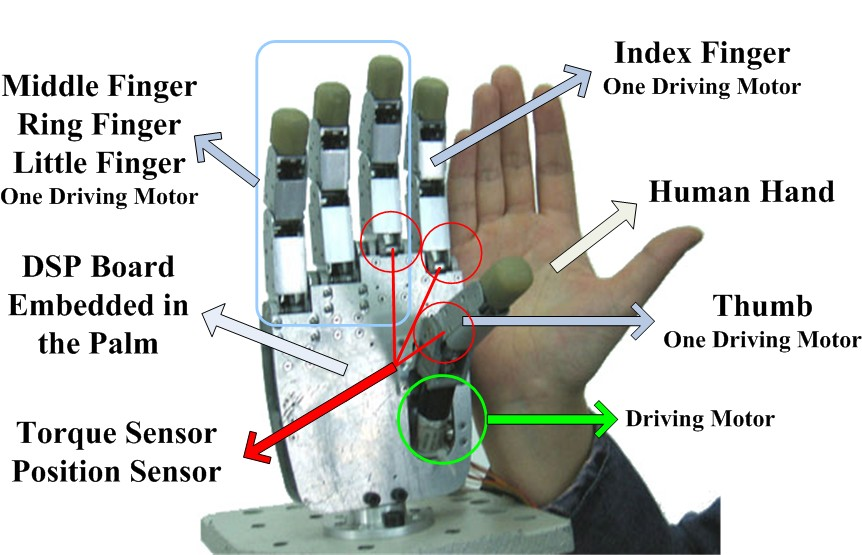
\includegraphics[height=3.3cm]{figs/DLR-Prothese}
  \end{tabular}
  \caption{(left) The DLR Hand II. (right) The DLR prosthetic hand.}
  \label{fig:DLRHandII}
\end{figure}

To this end, two types of interfaces between the patient and the
prosthesis have been developed or are being studied:
\emph{invasive} and \emph{non-invasive}.
%% The former involve
%% control based upon signals gathered directly from the user's nervous
%% system, either via brain implants or surgical use of
%% electrodes. Invasive interfaces are supposed to guarantee a higher
%% signal quality as far as control is concerned, but involve
%% surgery. Non-invasive interfaces are easier to handle, manufacture and
%% implant, but require a much better signal conditioning, since they
%% usually work with surface (skin) signals or vision and gaze tracking.
In the context of non-invasive interfaces for controlling mechanical
hands, a concrete possibility arises from \emph{forearm surface
electromyography (EMG)} \cite{zecca}, a technique by which muscle
activation potentials are gathered by electrodes placed on the
patient's forearm skin; these potentials can be used to track what
muscles the patient is activating, and with what force.  Still, the
EMG signal suffers from a number of problems, among which the
placement of the electrodes, signal drifting and change due to sweat
formation and muscular fatigue and cross-talking among deep and
superficial muscles. See \cite{deluca} for an overview of the problems
posed by this signal. In this paper, we pursue the approach based upon
\emph{machine learning} techniques already attempted in, e.g.,
\cite{dunlop,fukuda,smagt}.
% Therefore
%we seek to approximate a map such as the one described above by
%choosing a function in a suitable functional space, based upon a
%number of example known values of the map, i.e., values gathered
%during an experimental phase called \emph{training}. If the choice
%is good, the unknown target values corresponding to further points
%in the input space (in this case, EMG potential values) can be
%predicted on-line (\emph{testing} phase), and the patient's
%intention to move a muscle can be reconstructed.

%We focus here upon the initial task of building such a map for an
%able-bodied subject, and in particularly controlled conditions. In a
%subsequent phase, it is hoped that it will be possible to use this
%method to actually drive a mechanical hand implanted on an
%amputee. There are concrete possibilities to do this, since a
%remarkable muscular and nerve activity can still be present in hand
%amputees forearms, also years after the amputation has taken place.

So far, in literature, machine learning applied to surface EMG has
been able to \emph{classify} finger movement only.  However,
control of the exerted force is crucial, for instance for holding
a hammer or grasping an egg. We show a detailed comparative
analysis of what machine learning can do when applied to such a
problem. Over two days, we have gathered forearm surface EMG data
while holding a force sensor with different finger combinations.
We have then trained three different machine learning systems to
compute, from the EMG signal, the finger movements and the finger
force. The three approaches we have experimented with are: $(a)$ a
simple feed-forward neural network with one hidden layer, $(b)$ a
Support Vector Machine with radial basis function kernel
\cite{BGV92}, $(c)$ Locally Weighted Projection Regression
\cite{lwpr}.
% All approaches were trained on a massive amount of
%data, but bearing in mind the following important point: in a real
%setting, that is, when a patient is required to train the
%prosthesis, training must eventually stop and the model so
%obtained must give good prediction results for a long
%time---picture the ideal scenario in which training happens in the
%first day of use, and then the prosthesis must be used in the
%following months or years by the same person.
%
%This has involved a careful analysis of the short- and medium-term
%changes in the EMG signal. In other words, the correct way of
%\emph{sampling in the input space in a reasonable amount of time}
%must be found.
Our numerical results indicate that, in such a scenario, the type of
grasp can be reconstructed with an average accuracy of $90\%$, and the
applied force can be predicted with an average percentage error of
$10\%$, meaning about $5$N over a range $50$N.
%% None of the tested
%% approaches clearly outperforms the others, which seems to indicate
%% that machine learning as a whole is a viable approach. All in all,
%% this looks highly encouraging in applying machine learning to enable
%% amputees gain a fine control over their prostheses.
